\documentclass[a4paper]{report} %padrao letterpaper, 10pt
\usepackage[utf8]{inputenc}
\usepackage{amsfonts,amssymb,graphicx,enumerate}
\usepackage[centertags]{amsmath}
\usepackage[lmargin=3cm,rmargin=3cm,tmargin=3cm,bmargin=3cm]{geometry}

\usepackage{setspace,cite}
\doublespacing
\renewcommand{\bibname}{Bibliografia}
%\usepackage[portuguese]{babel}
\usepackage{identfirst}


\newenvironment{dem}[1][Demonstra\c c\~ao]{\textbf{#1:}\

}  {\hfill\rule{1ex}{1ex}}
%*******************************************************
% Definindo novos comandos
\providecommand{\sin}{} \renewcommand{\sin}{\hspace{2pt}\textrm{sen}}
\newcommand{\R}{\mathbb{R}} %simbolos de numeros reais
%*******************************************************
\title{\textbf{Laboratório Nacional de Computação Científica}\\
Relat\'orio de Atividades PIBIC\\ 
Processo CNPq \hspace{0.2 cm} 153399/2015-5\\
\vspace{2cm}
\begin{center}
	%
\includegraphics[scale=0.7]{figures/lncc}
	%\hspace{0.3cm}
	%
\includegraphics[scale=0.15]{figures/faeterj}
	%\hspace{0.3cm}	
	%
\includegraphics[scale=0.25]{figures/cnpq}
\end{center}
}
%\author{\textbf{}}

\date{}    %para ocultar a data digite: \date{ }
%*******************************************************
\begin{document}    %Inicio do documento
\maketitle  %cria o titulo na capa

%%%%%%%%%%%%%%%%%%%%%%%%%%%%%%%%%%%%%%%%%%%%%%%%%%%%%%%%%%%%%%%%%%%%%%%%%%%%%%%%
\section*{Dados Gerais}

Este documento é uma descrição das pesquisas feitas pelo bolsista \textbf{Oscar Neiva Eulálio Neto} (CPF 140.409.757-07) para o Programa de Bolsas de Iniciação Científica (PIBIC) do Laborat\'orio Nacional de Computa\c{c}\~ao Cient\'ifica (LNCC). O trabalho possui como título: \textbf{Controle e Simulação de Sistemas Sujeitos a Saltos Markovianos} e os estudos foram supervisionados pelo professor Marcos Garcia Todorov, pesquisador da instituição.

  
%%%%%%%%%%%%%%%%%%%%%%%%%%%%%%%%%%%%%%%%%%%%%%%%%%%%%%%%%%%%%%%%%%%%%%%%%%%%%%%%
\section*{Introdução}

A crescente quantidade de informação na \textit{Web} nos últimos anos, fez das ferramentas de busca algo indispensável na coleta de informação. O algoritmo \textit{PageRank} é a técnica chave do Google, proposta inicialmente em \cite{brin2012reprint} no ano de 1998. O Google é um dos mais bem sucedidos buscadores e o \textit{PageRank} é com certeza um dos fatores deste sucesso.

Para o cálculo do \textit{PageRank} algumas considerações devem ser feitas e um fator crítico a ser levado em conta é o tamanho da estrutura da \textit{Web}. A \textit{Web} até 2010 era composta por pouco mais de 8 bilhões de páginas \cite{ishiiTAC10}, lembrando ainda que esse número está em constante crescimento. Atualmente a estimação do \textit{Ranking} das páginas é feita de forma centralizada no Google, onde toda a coleta de dados da \textit{Web} é feita por rastreadores, ou \textit{Crawlers}, que a acessam de forma autônoma.

O algoritmo do \textit{PageRank} está associado a conceitos da área de sistemas e controle. Seu cálculo dá-se por uma equação de diferença \cite{pagerankSIREV}, cuja a matriz de transição é do tipo estocástica, devido a possibilidade do conjunto de páginas da \textit{Internet} poderem ser modeladas como uma cadeia de Markov de estados discreto \cite{costafragosomarques}.

O trabalho tratou-se de uma revisão dos modelos propostos para o algoritmo do \textit{PageRank} em \cite{ishii2014pagerank}. Assim, inicialmente foi necessário um estudo dos conceitos por trás dos modelos matemáticos do algoritmo, para que em seguida pudessem ser realizadas as simulações e serem feitas conclusões a partir delas. Foram realizadas simulações desde os modelos mais simples a aqueles que estão associados a situações mais mal comportadas. Por fim, foram analisados os resultados e comparados os modelos e recursos usados nas simulações.


%%%%%%%%%%%%%%%%%%%%%%%%%%%%%%%%%%%%%%%%%%%%%%%%%%%%%%%%%%%%%%%%%%%%%%%%%%%%%%%%
\section*{O Algoritmo \textit{PageRank}}

O \textit{PageRank} é o principal algoritmo por trás das engrenagens de busca do \textit{Google}, criado em 1998 por Lawrence Page e Sergey Brin (figura \ref{larry}) para atribuir pesos a páginas da \textit{Web}. Ele tem como função atribuir um valor numérico para cada elemento em um conjunto de documentos, em que na \textit{Internet} tratariam-se de páginas \textit{Web}. Tendo como principal objetivo a identificação das páginas mais importantes aos usuários da rede, de forma a atribuir valores maiores as páginas mais importantes.

\
\begin{figure}[!htb]
	\centering
	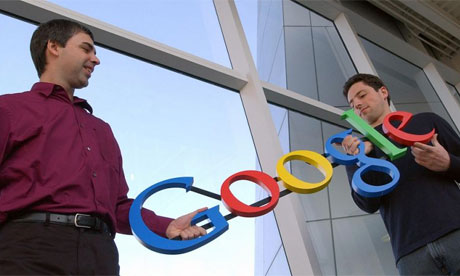
\includegraphics[scale=0.45]{imagens/larry}
	\caption{Lawrence Page e Sergey Brin criadores do \textit{PageRank} e fundadores do Google.}
	\label{larry}
\end{figure}

%O grau de importância das páginas
A respeito da atribuição de importância às páginas, a página mais importante será a mais visitada e a página mais visitada será aquela que está associada a um maior número de \textit{links}. De forma mais precisa o número de visitas de uma página vai estar associado aos \textit{links} de saída que ela possui. Contudo, uma página também pode ser considerada importante por estar próxima a uma página de alto \textit{PageRank}.


%%%%%%%%%%%%%%%%%%%%%%%%%%%%%%%%%%%%%%%%%%%%%%%%%%%%%%%%%%%%%%%%%%%%%%%%%%%%%%%%
\subsection*{O Problema do \textit{PageRank}}

%Apresentação do modelo simples
O \textit{PageRank} pode ser pensado como um modelo que simula o comportamento de um usuário que age de forma aleatória. Considerar que existe um navegador que vai acessando páginas aleatoriamente, de forma a clicar somente em \textit{links} na página em que se encontra, consiste no modelo mais simples de cálculo do \textit{PageRank}. 

%Problema 1 - Buraco negro
Outra importante situação que precisa ser levada em consideração é a possibilidade de um usuário acessar uma página sem links de saída, como por exemplo, um link que o direcione para um documento PDF, como ilustrado na figura \ref{blackhole}. Neste caso o usuário poderia usar o botão de voltar do \textit{Browser} para sair deste tipo de buraco negro na rede, o que simplifica possíveis problemas no cálculo do \textit{PageRank}.  

\
\begin{figure}[!htb]
	\centering
	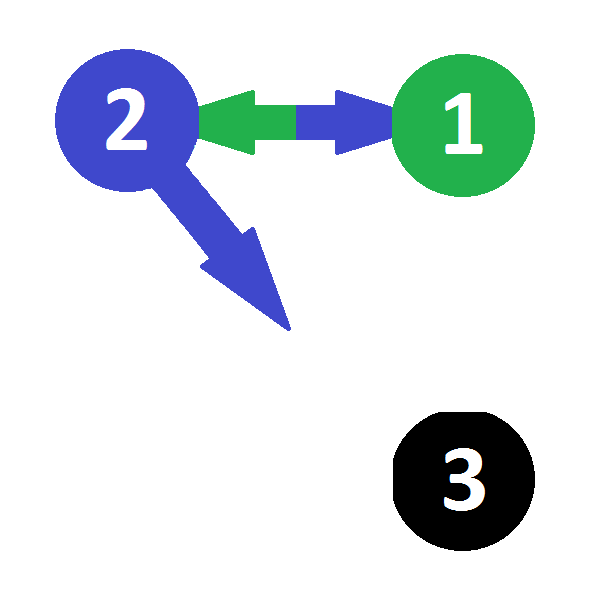
\includegraphics[scale=0.3]{imagens/blackhole1}
	\hspace{0.1cm}
	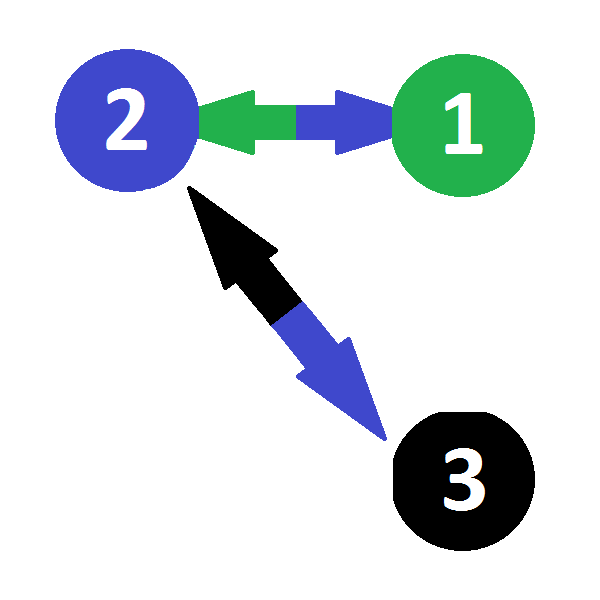
\includegraphics[scale=0.3]{imagens/blackhole2}
	\caption{O buraco negro da \textit{Web}.}
	\label{blackhole}
\end{figure}

%Problema 2 - Teleportation Model
Um outro problema surge ao considerar-se que o usuário pode saltar de uma página para outra sem seguir a estrutura de \textit{links}, por ficar entediado, ou por um outro motivo qualquer. Um exemplo de como isso poderia ocorrer, é o caso do usuário estar na página do Laboratório Nacional de Computação Científica - LNCC e seguindo a estrutura de \textit{Hyperlink}, clicar em um \textit{link} que o leve à página do governo federal. No entanto, o usuário de repente altera o \textit{Uniform Resource Locator - URL} e vai para um \textit{site} de notícias que não está diretamente ligado aos outros dois \textit{sites}. Este exemplo é ilustrado na figura \ref{tele}.

\
\begin{figure}[!htb]
	\centering
	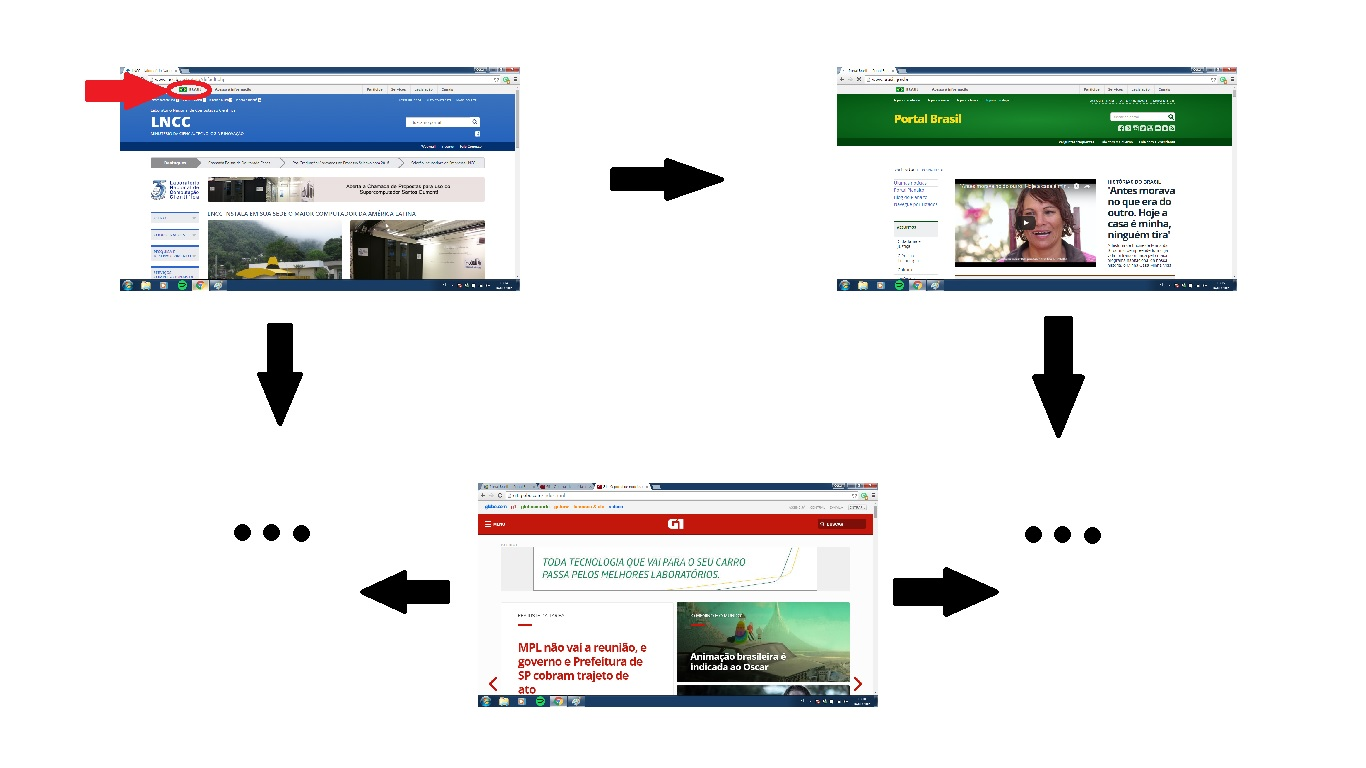
\includegraphics[scale=0.3]{imagens/tele}
	\caption{Navegação entre páginas indiretamente conectadas.}
	\label{tele}
\end{figure}

%Problema 3 - A massividade da Web
A massividade da \textit{Web} é uma das principais questões por trás do cálculo do \textit{PageRank}, considerando que a dimensão da \textit{Web} pode tornar o ranqueamento de páginas impossível. No entanto, a solução para este problema é o uso de algoritmos distribuídos, sobre os quais a cada ano novas publicações são feitas \cite{lei2015distributed}. Neste contexto, a fim de melhorar a performance do processamento, o cálculo a partir do modelo distribuído é realizado com a ajuda de vários conputadores num \textit{cluster}, como o da figura \ref{cluster}.  

\
\begin{figure}[!htb]
	\centering
	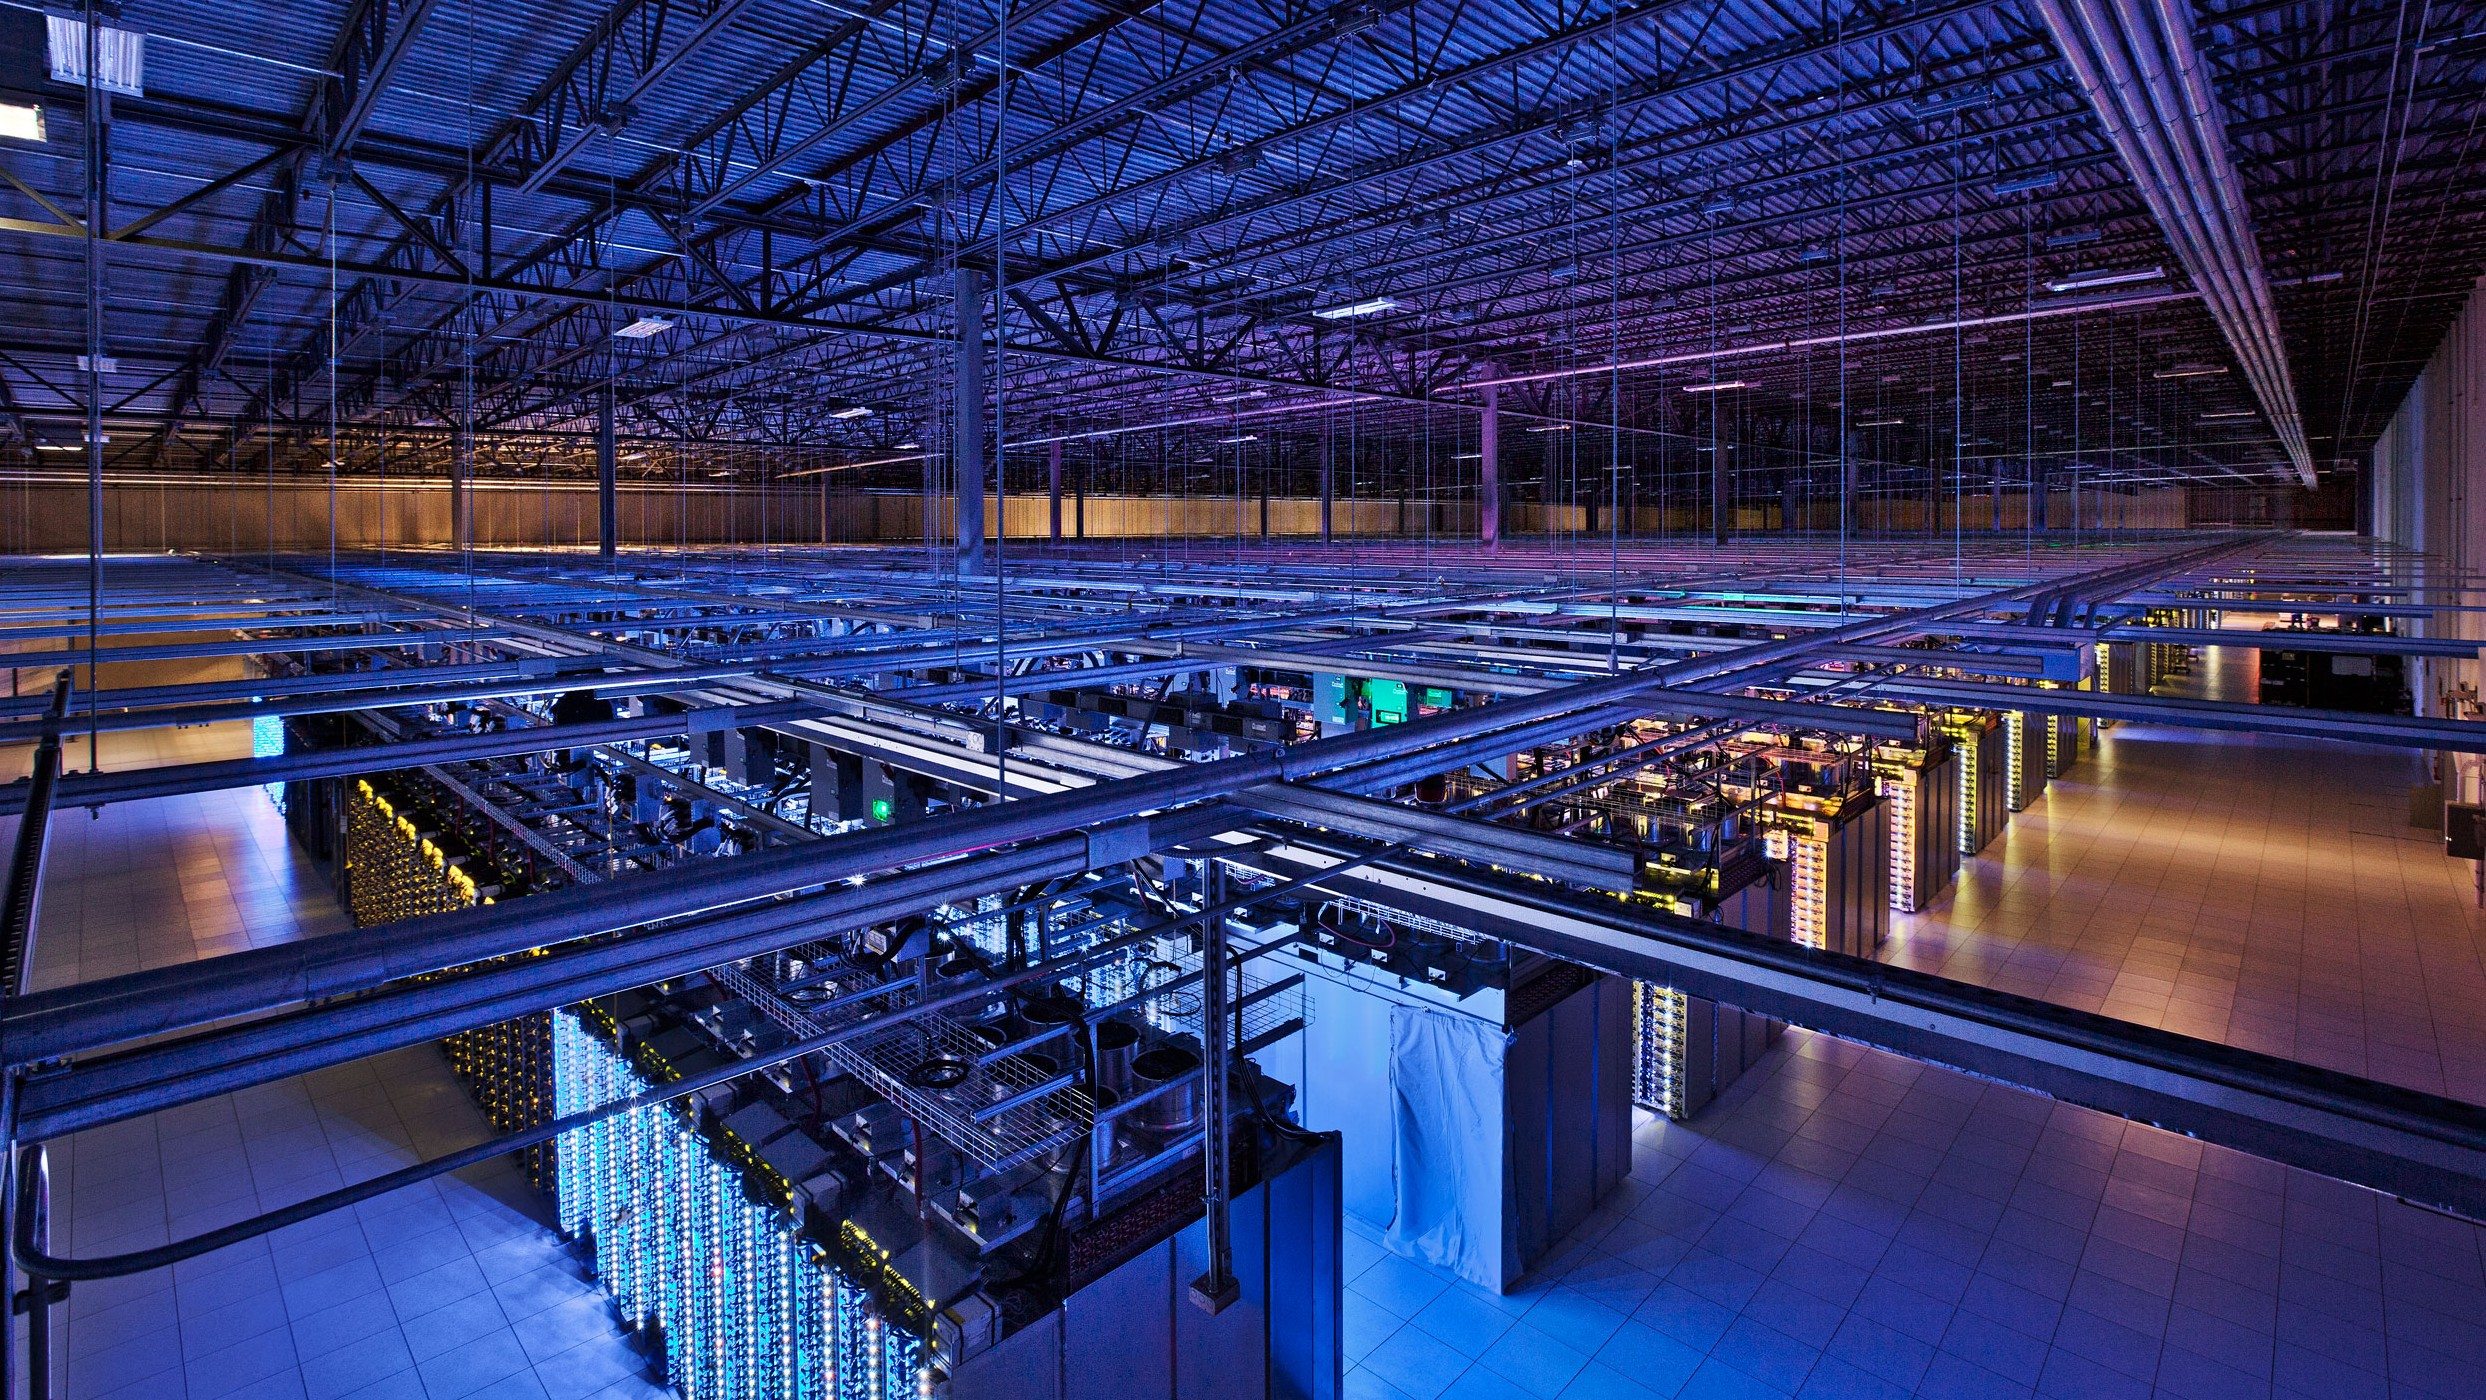
\includegraphics[scale=0.1]{imagens/cluster}
	\caption{Cluster do Google.}
	\label{cluster}
\end{figure}

%%%%%%%%%%%%%%%%%%%%%%%%%%%%%%%%%%%%%%%%%%%%%%%%%%%%%%%%%%%%%%%%%%%%%%%%%%%%%%%%
\section*{Definição dos Modelos}

%%%%%%%%%%%%%%%%%%%%%%%%%%%%%%%%%%%%%%%%%%%%%%%%%%%%%%%%%%%%%%%%%%%%%%%%%%%%%%%%
\subsection*{A Matriz \textit{Hyperlink}}

A construção da matriz \textit{hyperlink} é feita com base na estrutura da \textit{Web}, ou ainda do grafo que a representa. Assim, considerando que o grafo da figura \ref{grafo} representa um conjunto de páginas interligadas, seus elementos são definidos da seguinte forma: 

\
\begin{figure}[!htb]
	\centering
	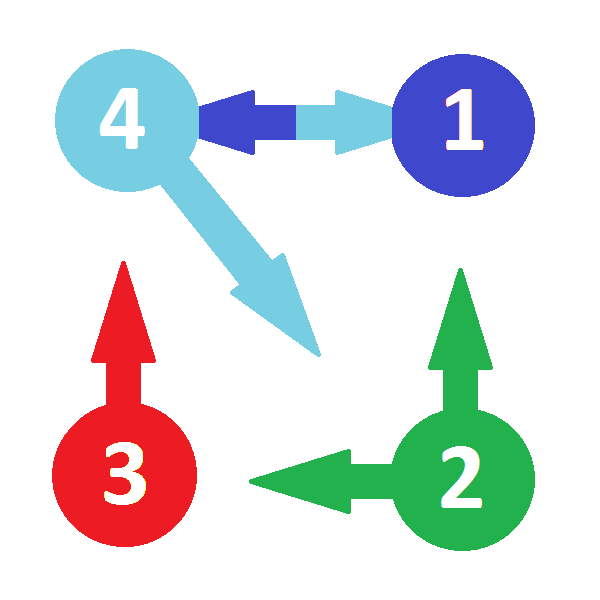
\includegraphics[scale=0.3]{imagens/grafo}
	\caption{Grafo representando \textit{links} entre páginas \textit{Web}.}
	\label{grafo}
\end{figure}

\begin{itemize}
\item $n$: como os n\'os, que representam as p\'aginas,

\vspace{0.1cm}
	
\item $\mathcal{E}$: como as arestas, que representam os \textit{links} entre as páginas.
\end{itemize}

Para representar o \textit{link} entre duas páginas específicas usa-se $i$ e $j$, de forma que o $i$ esteja associado à página de saída e $j$ com a de entrada. Considerando então o caso de um v\'ertice $i$ estar conectado a um $j$, tem-se $(i,j) \in \mathcal{E}$.

A matriz de transição que é construída a partir do grafo tem a seguinte propriedade para cada um de seus elementos:

\begin{equation}\label{a}
a_{ij} = \begin{cases}
\dfrac{1}{n_i}, & \text{caso}\, (i,j)\in \mathcal{E},\\
0, & \text{caso contr\'ario}.
\end{cases}
\end{equation}	

Cada elemento $a_{ij}$ é formado a partir das relações entre os nós do grafo. Para o nó $1$ por exemplo, constata-se que ele só possui relações com o nó $4$, por tanto, para um navegador que encontra-se em $1$ tem-se $100\%$, de certeza de que seu próximo passo será para $4$. Já no caso do nó $2$ pode-se observar que o navegador pode ir para $1$ ou $3$, ou seja, ele tem $50\%$ de chance de ir para cada um desses dois nós.

\begin{equation}\label{A}
A = \begin{pmatrix}
 0 & 1/2 & 0 & 1/2 \\
 0 &  0  & 0 & 1/2 \\
 0 & 1/2 & 0 &  0  \\
 1 &  0  & 1 &  0
\end{pmatrix}
\end{equation}

E assim constroi-se a matriz de transição \eqref{A} de forma que todas as suas colunas respeitem a propriedade:

\begin{equation}\label{n}
\sum^{n}_{i=1} x_{i} = 1.
\end{equation}

%%%%%%%%%%%%%%%%%%%%%%%%%%%%%%%%%%%%%%%%%%%%%%%%%%%%%%%%%%%%%%%%%%%%%%%%%%%%%%%%
\subsection*{O \textit{Power Method}}

Este é o modelo mais simples para a estimação do \textit{PageRank}. Esta abordagem constitui-se de uma equação de diferença, a qual possui uma matriz de transição coluna estocástica e um vetor estocástico. O vetor estocástico é formado pelos valores das variáveis aleatórias da cadeia de Markov, ou seja os valores das páginas. O valor de \textit{PageRank} de um conjunto de $n$ páginas da \textit{Web} é definido como o vetor $x \in \mathbb{R}^{n \times 1}$ que satisfaz as seguintes equações:

\begin{equation}	
x = Ax, \quad x\geq0, \quad \sum^{n}_{i=1} x_{i} = 1, 
\end{equation}

\noindent onde $A \in \mathbb{R}^{n \times n}$ é a transposta da matriz de transição da cadeia de Markov.

Assim, o método usual para obtenção do \textit{PageRank} é o chamado \textit{Power Method} \cite{ishii2014pagerank}, que alcança o \textit{PageRank} através da seguinte iteração:

\begin{equation}
x(k+1) = Ax(k), \quad k\geq0, \quad \text{com} \quad x(0) = x_0,
\end{equation}

\noindent onde $x_0 \in \mathbb{R}^{n \times 1}$ é uma condição inicial positiva de soma igual a um.


%%%%%%%%%%%%%%%%%%%%%%%%%%%%%%%%%%%%%%%%%%%%%%%%%%%%%%%%%%%%%%%%%%%%%%%%%%%%%%%%
\subsubsection*{Questões de Convergência do \textit{Power Method}}

Após um número considerável de iterações e em um número considerável de casos, o \textit{Power Method} atinge a distribuição limite com os valores de \textit{PageRank} de cada página. Além disso, independente da condição inicial, ao final das iterações os valores de \textit{PageRank} tendem a ser os mesmos.

Isso ocorre devido a matriz de transição ser irredutível, o que reflete no navegador aleatório sempre conseguir chegar a uma certa página partindo de uma outra qualquer, mesmo que essas duas páginas não estejam diretamente conectadas. Observando o grafo da figura \ref{grafo}, pode-se observar que não existe um \textit{link} direto entre $1$ e $3$, para chegar-se em $3$ a partir de $1$ o usuário teria de ir de $1$ para $4$, de $4$ para $2$ e de $2$ para $3$.


%%%%%%%%%%%%%%%%%%%%%%%%%%%%%%%%%%%%%%%%%%%%%%%%%%%%%%%%%%%%%%%%%%%%%%%%%%%%%%%%
\subsection*{O \textit{Teleportation Model}}

O \textit{Teleportation Model} é uma estratégia reconhecida para que, através de uma pequena modificação na matriz $A$, o método convirja globalmente para o PageRank. Essa modificação na matriz $A$ é representada como uma combinação convexa de duas matrizes, em que a matriz de transição agora passa a ser $M$, dada por:

\begin{equation}
M = (1-m)A + \frac{m}{n}{\bf11}^T,
\end{equation}

\noindent onde $M \in \mathbb{R}^{n \times n}$, $m \in (0,1)$ e $\textbf{1} \in \mathbb{R}^{N \times 1}$. Em que $\textbf{11}^T$ é uma matriz preenchida de 1's, resultante do produto entre um vetor de 1's $\textbf{1}$ e um vetor de 1's transposto $\textbf{1}^T$. Vale lembrar também que $n$ é o número de nós do grafo, ou número de páginas, e que $A$ continua sendo a mesma matriz de transição, apenas é substituida por $M$ na equação apresentada no \textit{Power Method}.


%%%%%%%%%%%%%%%%%%%%%%%%%%%%%%%%%%%%%%%%%%%%%%%%%%%%%%%%%%%%%%%%%%%%%%%%%%%%%%%%
\subsection*{O Modelo dos Algoritmos Distribu\'idos}

A fim de tornar o cálculo do \textit{PageRank} menos custoso, e melhor explorar os recursos computacionais dos servidores disponíveis na web, uma alternativa é o emprego de algoritmos distribuídos. A agregação de tais experimentos aleatórios faz então com que o \textit{power method} se torne um sistema linear com saltos Markovianos do seguinte tipo:

\begin{equation}
	x(k+1) = A_{\theta(k)}x(k), \quad k\geq0, \quad \text{com} \quad x(0) = x_0. 
\end{equation}

Em que a matriz de transição $A$ agora passa a ser várias matrizes \textit{links} distribu\'idas $A_i \in \mathbb{R}^{n \times n}, \: i = 1,2, ..., n$. Sendo cada uma das matrizes distribuídas definidas da seguinte forma: 

\begin{itemize}
\item a i-ésima coluna de $A_i$ coincide com a i-ésima coluna de $A$,
\item a j-ésima entrada diagonal de $A_i$ é igual a um,
\item para $j = 1, ..., n, \: j \neq i$, todas as outras entradas $a_{ij}$ são iguais a zero.
\end{itemize}

A ideia agora é de que cada página fará o seu cálculo de \textit{PageRank}, por isso são criadas as matrizes  distribuídas. Em que as matrizes são construídas da seguinte forma.

\begin{equation}\label{A12}
A_1 = \begin{pmatrix}
 0 &  0  & 0 &  0 \\
 0 &  1  & 0 &  0 \\
 0 &  0  & 1 &  0  \\
 1 &  0  & 0 &  1
\end{pmatrix}
%
\hspace{0.5cm}
%
A_2 = \begin{pmatrix}
 1 & 1/2 & 0 &  0 \\
 0 &  0  & 0 &  0 \\
 0 & 1/2 & 1 &  0  \\
 0 &  0  & 0 &  1
\end{pmatrix}
\end{equation}

\vspace{0.1cm}

\begin{equation}\label{A34}
A_3 = \begin{pmatrix}
 1 &  0  & 0 &  0 \\
 0 &  1  & 0 &  0 \\
 0 &  0  & 0 &  0  \\
 0 &  0  & 1 &  1
\end{pmatrix}
%
\hspace{0.5cm}
%
A_4 = \begin{pmatrix}
 1 &  0  & 0 & 1/2 \\
 0 &  1  & 0 & 1/2 \\
 0 &  0  & 1 &  0  \\
 0 &  0  & 0 &  0
\end{pmatrix}
\end{equation}	

Acoplando agora o modelo das matrizes distribuídas ao modelo do \textit{Teleportation} tem-se \eqref{Ax},

\begin{equation} \label{Ax}
x(k+1) = (1 - \hat{m})A_{\theta(k)}x(k) + \frac{\hat{m}}{N} \textbf{11}^T, \quad k \geq 0, \quad \text{com} \quad x(0) = x_0,
\end{equation}

\noindent onde $\hat{m}$ é definido como: 

\begin{equation}\label{m}
\hat{m} = \frac{2m}{n-m(n-2)},
\end{equation}

\noindent e $m = 0.15$, é um parâmetro que foi obtido através de testes em \cite{zaki2012detection}.    

%%%%%%%%%%%%%%%%%%%%%%%%%%%%%%%%%%%%%%%%%%%%%%%%%%%%%%%%%%%%%%%%%%%%%%%%%%%%%%%%
\subsubsection*{Questões de Convergência do Modelo Distribuído}

De forma similar ao que ocorre no \textit{Power Method}, este método apresenta problemas de convergência, pois as matrizes $A_1$, $A_2$, $A_3$ e $A_4$ não são irredutíveis. Isso ocorre devido a inserção de 1's nas diagonais, o que na prática implicaria no nó $4$ só ter saída e chegada nele mesmo. Dessa forma, usando-se da matriz $A_1$, por exemplo, um navegador aleatório que partisse de $4$, nunca sairia de lá.

Para isso é usada uma média no tempo, em que a cada iteração é feita uma média de todos os estados anteriores. Assim $y(k)$ é a média do conjunto de amostras $x(0),... , x(k)$ definida como \eqref{y}, 

\begin{equation}\label{y}
y(k) = \frac{1}{k+1} \sum_{l=0}^{k} x(l).
\end{equation} 

\noindent De tal forma que o algoritmo converge no sentido da média quadrada, ou seja,

\begin{equation}\label{E}
\lim_{k\rightarrow \infty} \mathbb{E} [\parallel y(k)-x^*\parallel^2] = 0.
\end{equation}

\noindent Neste contexto, quanto maior for o número de iterações $k$, mais o valor de $y(k)$ se aproxima da
distribuição limite, o que representa o valor de \textit{PageRank}.

A fim de minimizar custos computacionais, um formato recursivo da média $y(k)$ foi usado nas simulações, que possui o seguinte formato:

\begin{equation}\label{yr}
	y(k+1) = \frac{(k+1)}{(k+2)}y(k) + \frac{1}{(k+2)}x(k+1).
\end{equation}

%%%%%%%%%%%%%%%%%%%%%%%%%%%%%%%%%%%%%%%%%%%%%%%%%%%%%%%%%%%%%%%%%%%%%%%%%%%%%%%%
\section*{Simulações}

As simulações foram feitas a partir dos modelos descritos anteriormente e a partir do grafo da figura \ref{grafoSimu} com o objetivo de observar algumas considerações feitas na literatura.

\begin{figure}[!htb]
	\centering
	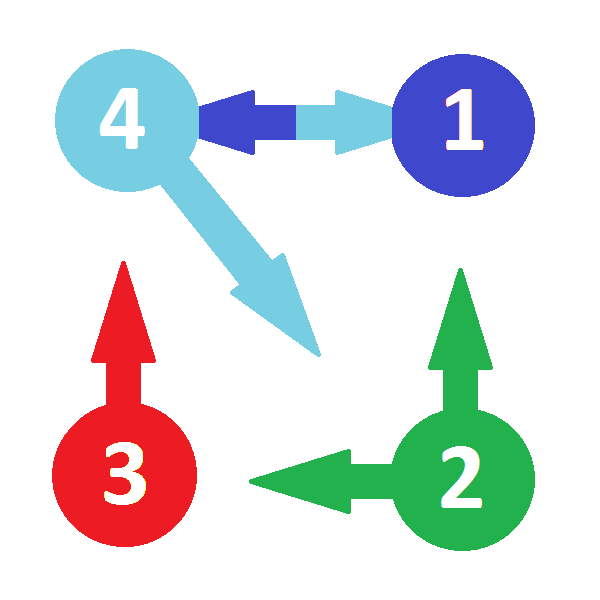
\includegraphics[scale=0.3]{imagens/grafo}
	\caption{Grafo usado nas simulações.}
	\label{grafoSimu}
\end{figure}

%%%%%%%%%%%%%%%%%%%%%%%%%%%%%%%%%%%%%%%%%%%%%%%%%%%%%%%%%%%%%%%%%%%%%%%%%%%%%%%%
\subsection*{Simulação do \textit{Power Method}}

Na simulação do modelo mais simples do cálculo do \textit{PageRank}, o \textit{Power Method}, observa-se uma rápida convergência para cada um dos valores do vetor de estados. Isso ocorre devido a dimensão do problema usado na simulação. As cores das linhas dos gráficos, que representam os resultados das simulações, seguem o mesmo esquema das cores do grafo na figura \ref{grafoSimu}. Desta forma, as linhas do gráfico estão associadas às páginas da seguinte forma: 

\begin{itemize}
\item página 1: azul escuro,
\item página 2: verde,
\item página 3: vermelho,
\item página 4: azul claro.
\end{itemize}

\
\begin{figure}[!htb]
	\centering
	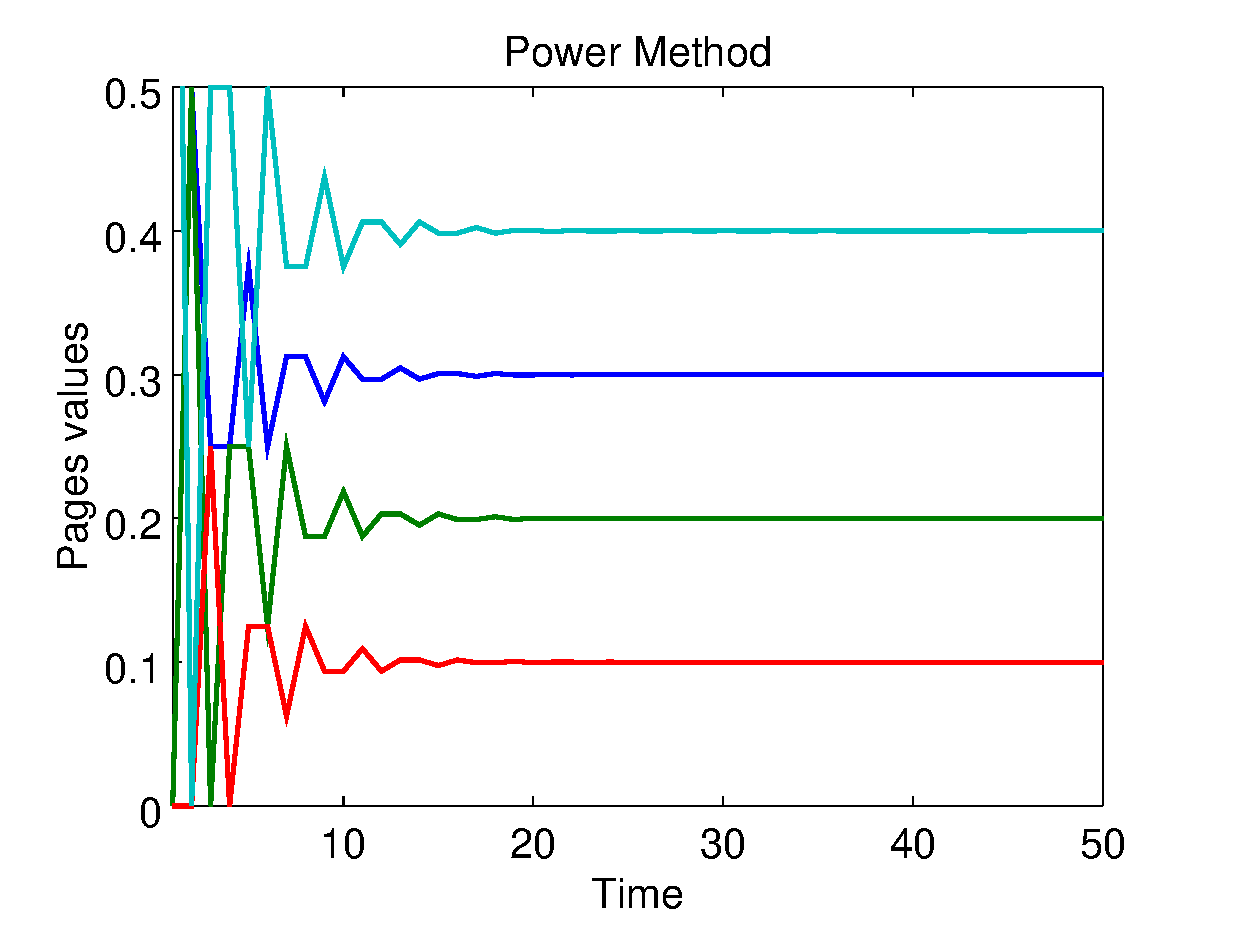
\includegraphics[scale=0.3]{imagens/powermethod}
	\caption{Resultado das simulações do \textit{Power Method}.}
	\label{powermethod}
\end{figure}

Assim pode-se observar que a página de número $4$ foi a que recebeu um maior \textit{PageRank}, dentro deste conjunto de páginas. Ao mesmo que $4$ é a página que está associada a um maior número de links, tanto de entrada quanto de saída, o que define seu alto valor de \textit{PageRank}.

Entretanto, um resultado em primeira vista parece não ser conveniente ao grafo. Ao analisar-se o valor final de $1$ observa-se que ele está na frente da página $2$, e $2$ possui mais \textit{links} de saída que $1$. Fazendo-se uma análise mais cuidadosa nota-se que $1$ possui \textit{links} de entrada e saída para $4$, ou seja por estar ligada a $4$ e por $4$ possuir alto \textit{PageRank}, o número de acessos a $1$ foi maior por estar próximo a uma página supostamente importante.  

%%%%%%%%%%%%%%%%%%%%%%%%%%%%%%%%%%%%%%%%%%%%%%%%%%%%%%%%%%%%%%%%%%%%%%%%%%%%%%%%
\subsection*{Simulação do \textit{Teleportation Model}}

Na simulação do \textit{Teleportation Model}, figura \ref{teleportation}, também observa-se uma rápida convergência como nos resultados da simulação do \textit{Power Method}.

\
\begin{figure}[!htb]
	\centering
	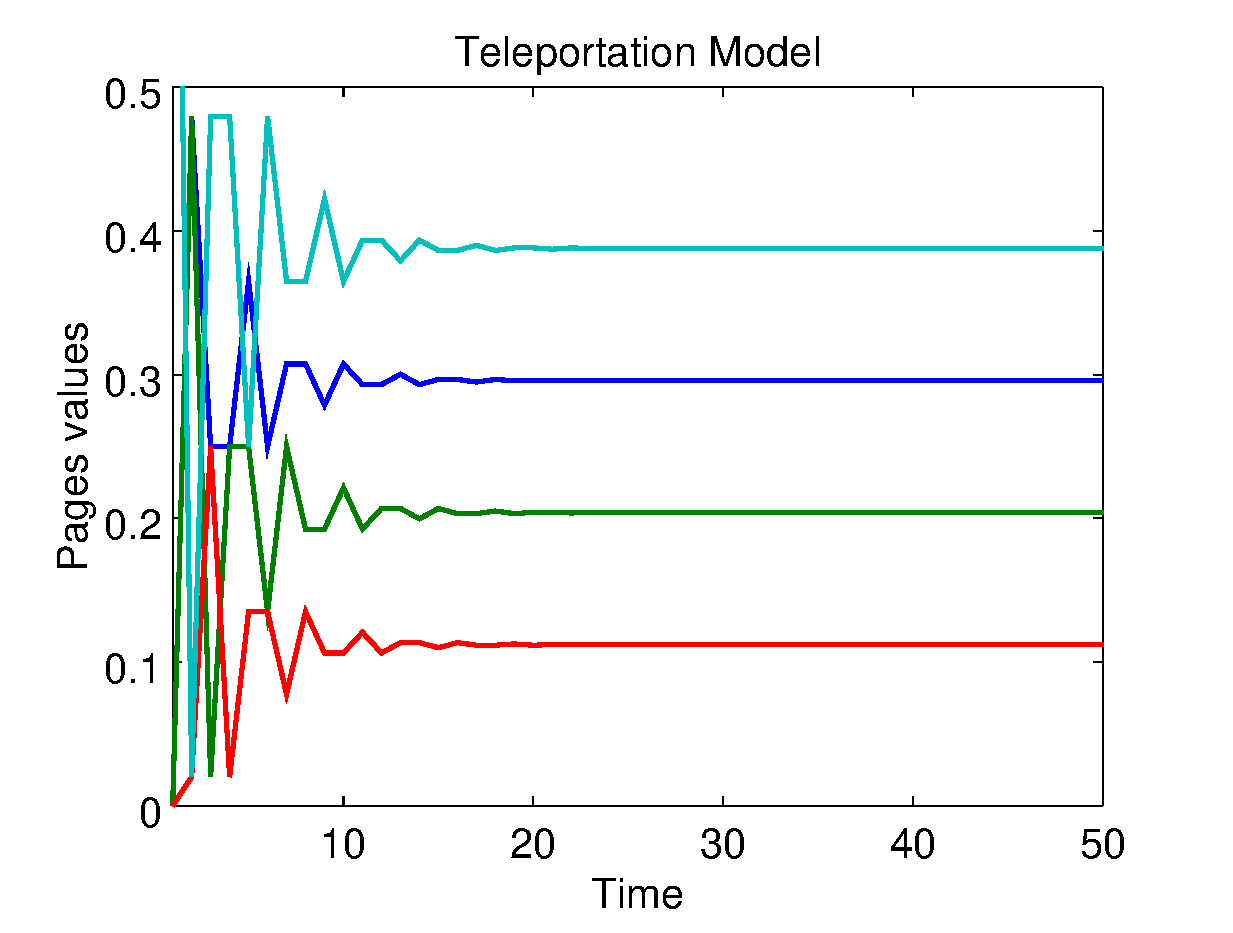
\includegraphics[scale=0.3]{imagens/teleportation}
	\caption{Resultado das simulações do \textit{Teleportation Model}.}
	\label{teleportation}
\end{figure}

Além disso uma grande semelhança é observada entre as duas simulações, como pode-se constatar na figura \ref{powertele}. Tanto a semelhança quanto a rápida convergência se devem ao fato do exemplo simulado não possuir um enorme número de estados $n$ e por ser bem comportado.

\
\begin{figure}[!htb]
	\centering
	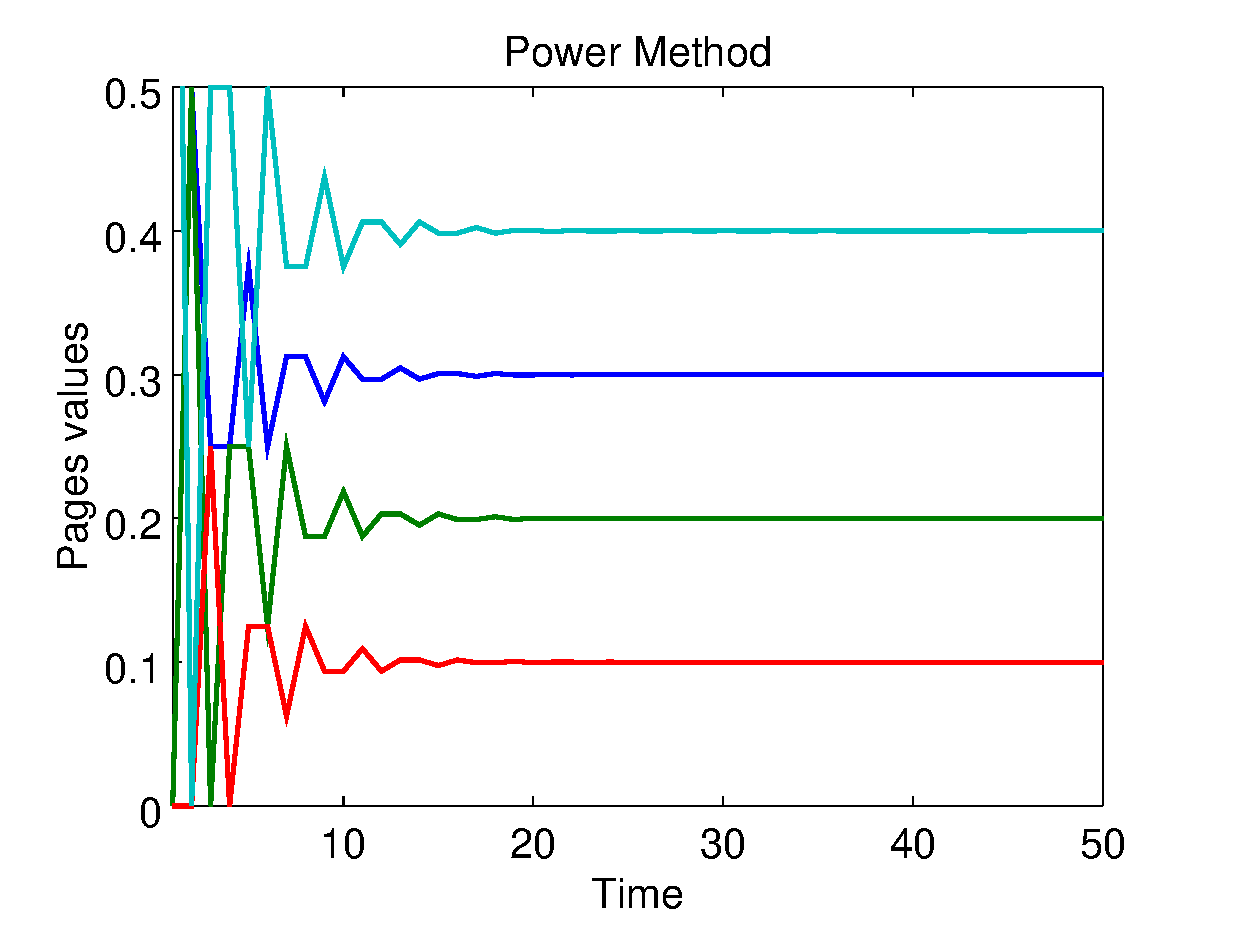
\includegraphics[scale=0.3]{imagens/powermethod}
	\hspace{0.1cm}
	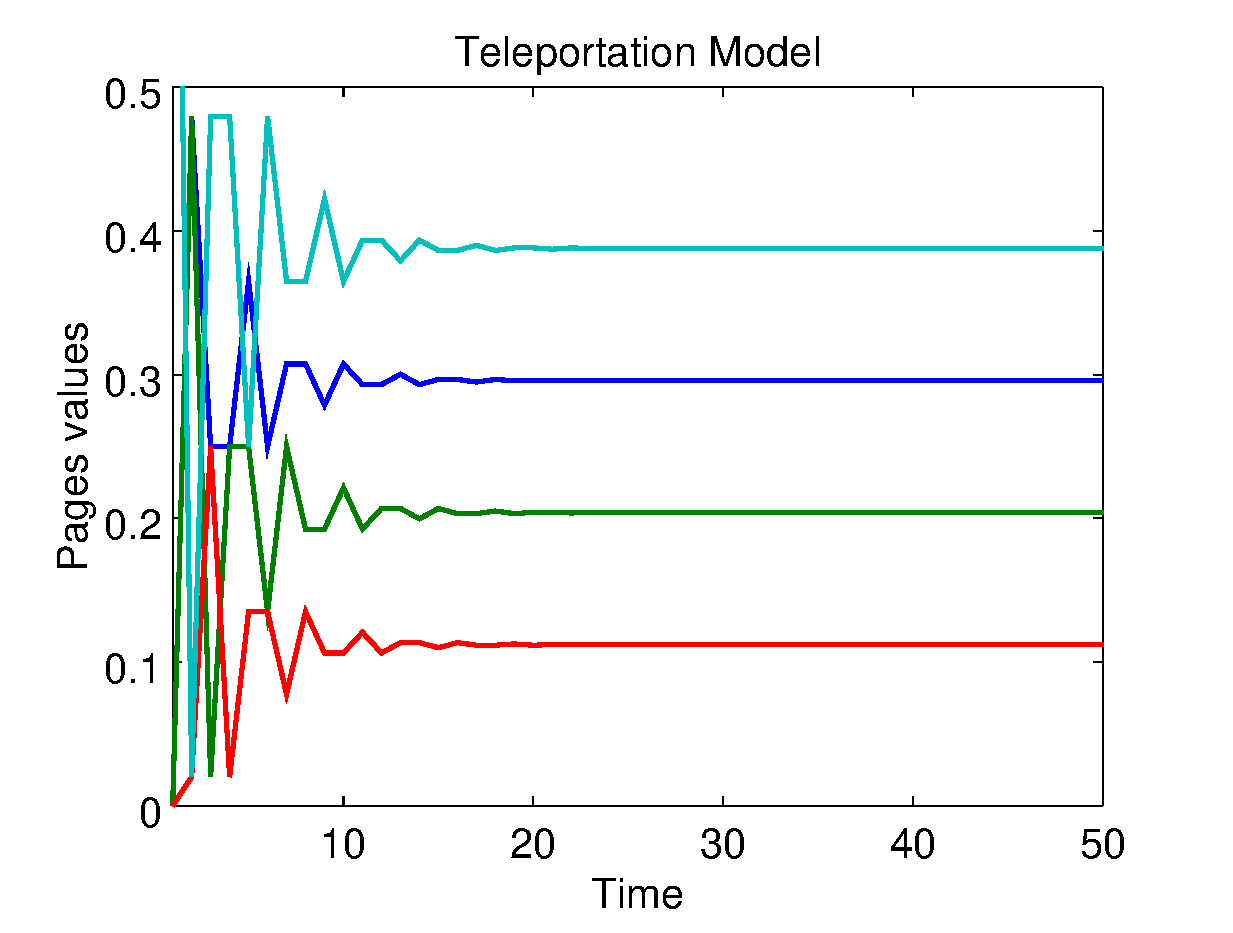
\includegraphics[scale=0.3]{imagens/teleportation}
	\caption{Comparação entre o \textit{Power Method} e o \textit{Teleportation Model}.}
	\label{powertele}
\end{figure}

%%%%%%%%%%%%%%%%%%%%%%%%%%%%%%%%%%%%%%%%%%%%%%%%%%%%%%%%%%%%%%%%%%%%%%%%%%%%%%%%
\subsection*{Simulações do Modelo Distribuído}

No modelo distribuído sem a média no tempo observa-se uma oscilação dos estados sem que os valores das variáveis aleatórias atinjam a distribuição limite, ou seja, neste modelo sem a média no tempo não foi possível encontrar um valor de \textit{PageRank} mesmo depois de $500$ iterações. Os resultados dessa simulação estão apresentados na figura \ref{teledistributed}.

\
\begin{figure}[!htb]
	\centering
	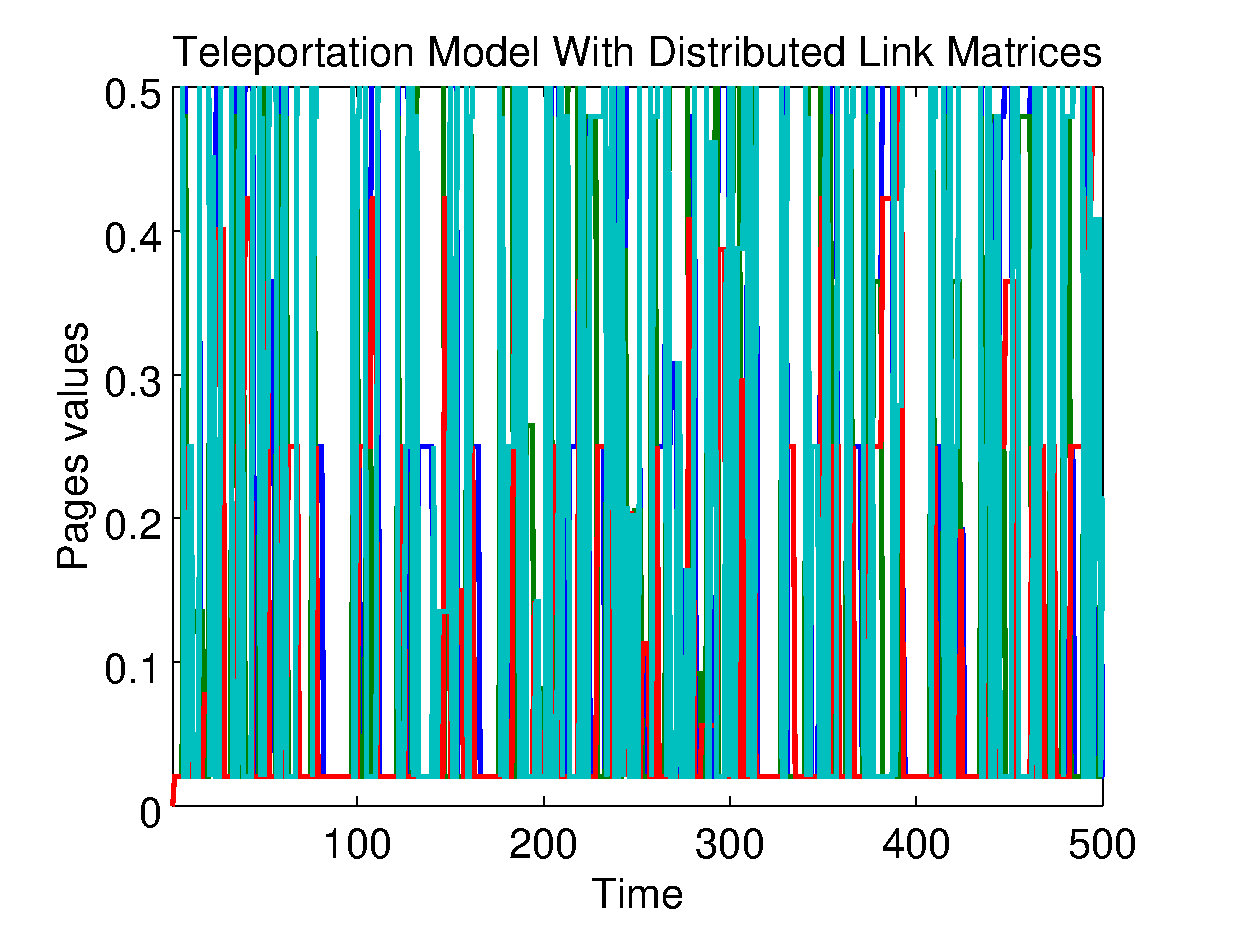
\includegraphics[scale=0.3]{imagens/teledistributed}
	\caption{Resultado das simulações do modelo distribuído.}
	\label{teledistributed}
\end{figure}

A não convergência ocorre devido as matrizes distribuídas possuirem 1's em suas diagonais, o que implicaria, por exemplo, usando-se a matriz $A_1$ como referência, nos nós $2$, $3$ e $4$ só terem saídas para si mesmo, seguindo o esquema apresentado na figura \ref{loop}.

\
\begin{figure}[!htb]
	\centering
	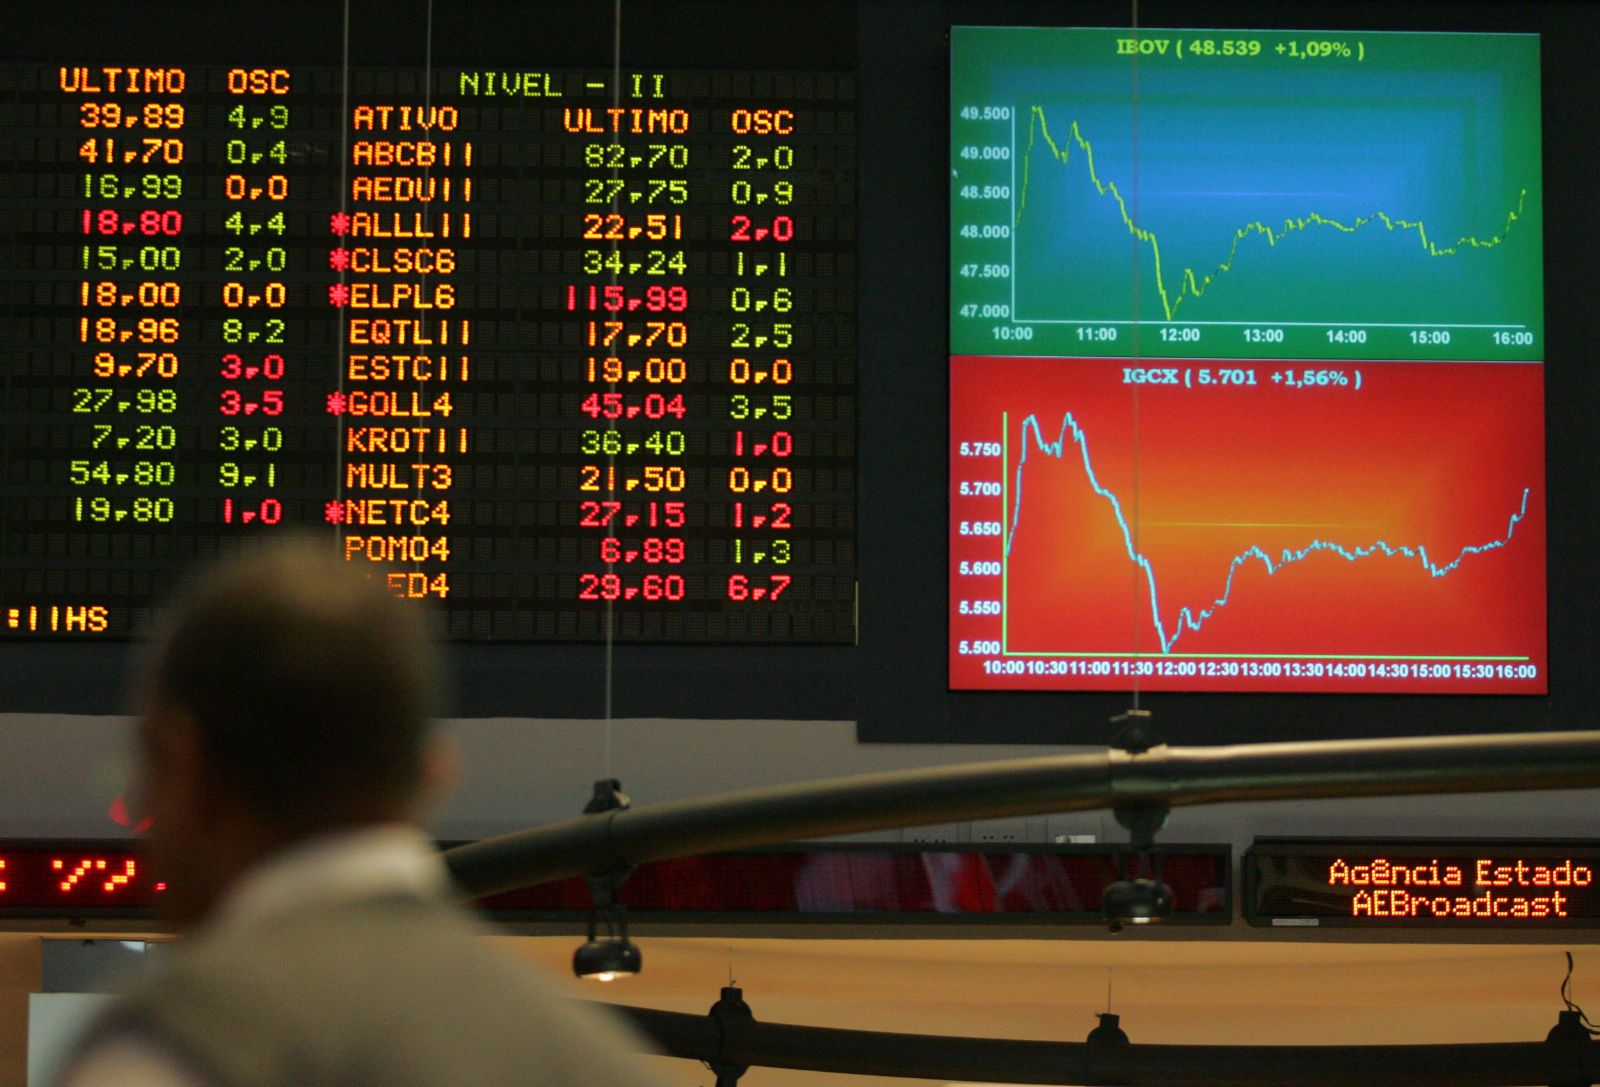
\includegraphics[scale=0.3]{imagens/loop}
	\caption{Abstração dos \textit{links} das páginas 2, 3 e 4 a partir da matriz $A_1$.}
	\label{loop}
\end{figure}

Entretanto, feita a média dos valores do modelo distribuído os resultados convergem, conforme é mostrado na figura \ref{timerecursive}. Mas ainda assim é possível observar algumas oscilações no gráfico, esta simulação também foi feita ao longo de $500$ iterações.

\
\begin{figure}[!htb]
	\centering
	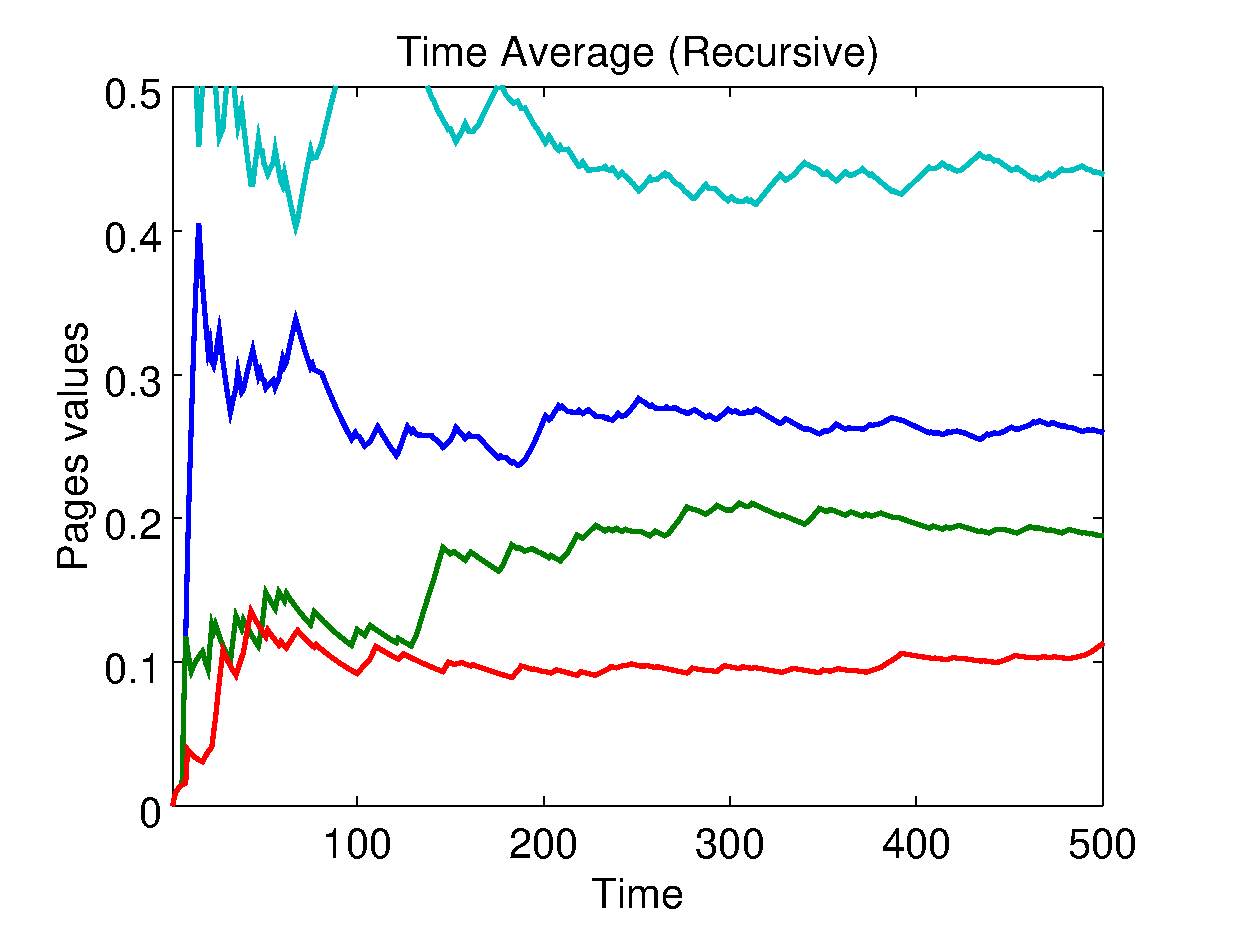
\includegraphics[scale=0.3]{imagens/timerecursive}
	\caption{Resultado das simulações do modelo distribuído com a média no tempo.}
	\label{timerecursive}
\end{figure}

Além disso, observa-se que na distribuição limite são atingidos valores bem próximos aos anteriormente encontrados para cada um dos estados no modelo do \textit{Power Method}, o que pode ser constatado a partir da figura \ref{powertime}.

\
\begin{figure}[!htb]
	\centering
	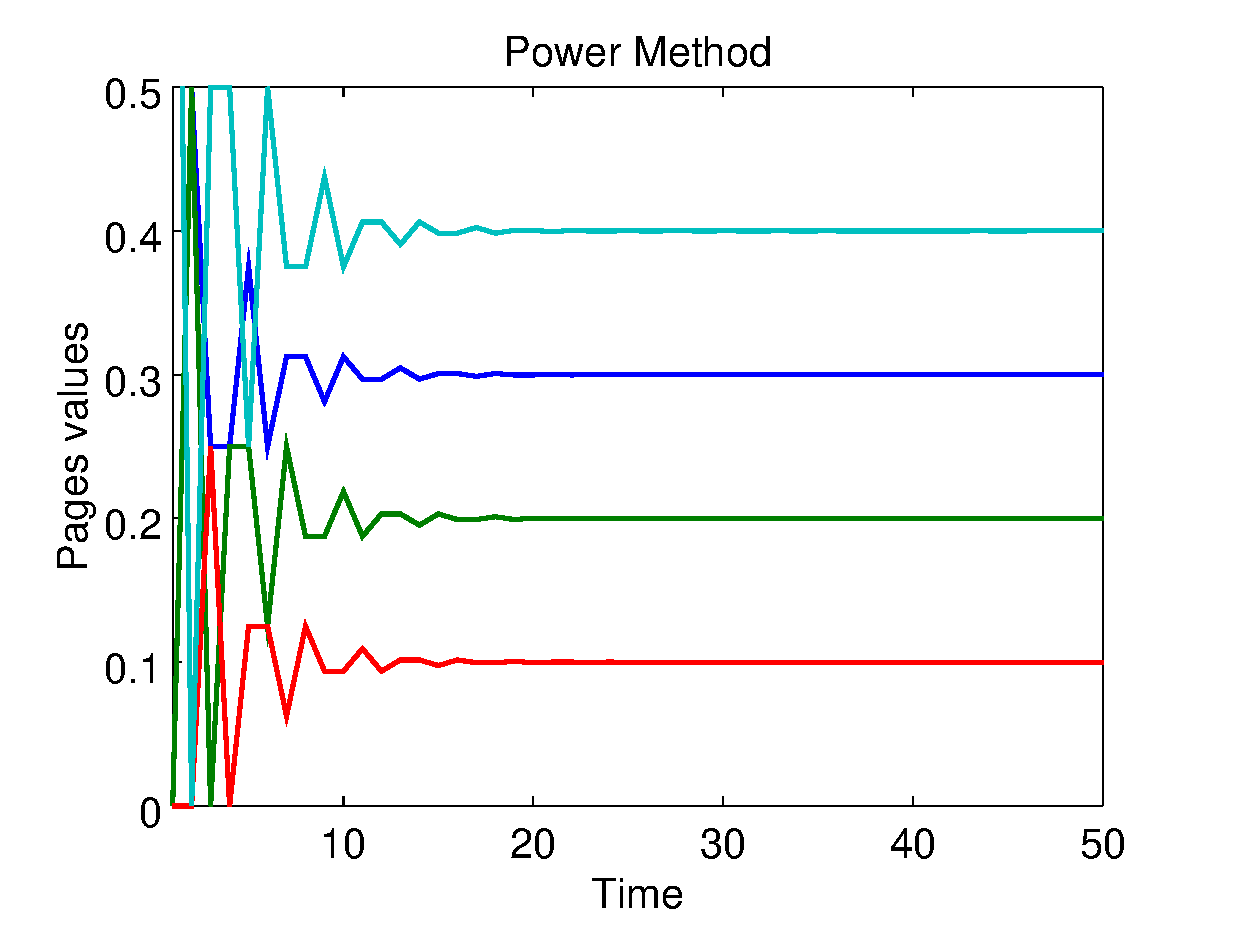
\includegraphics[scale=0.3]{imagens/powermethod}
	\hspace{0.1cm}
	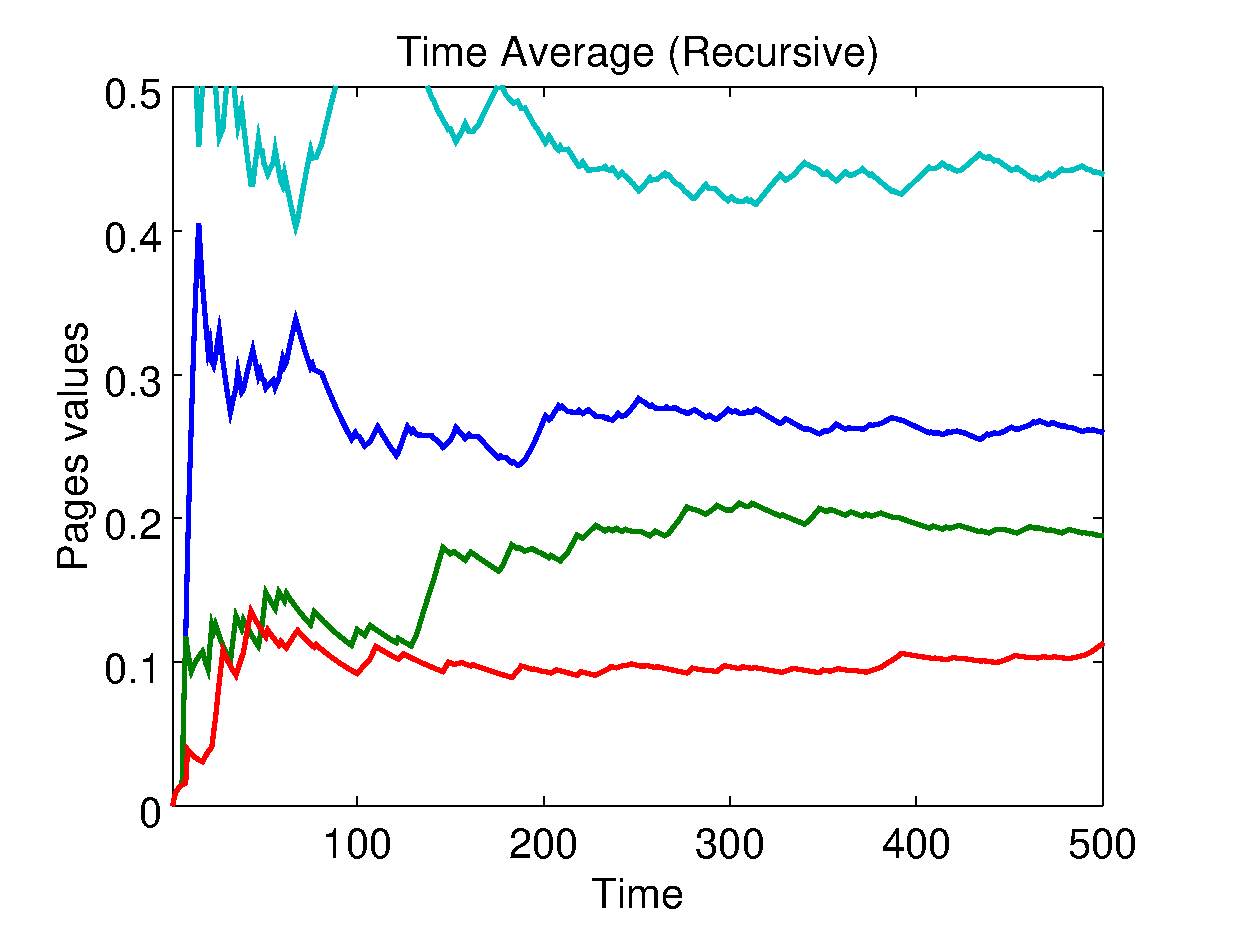
\includegraphics[scale=0.3]{imagens/timerecursive}
	\caption{Comparação entre o \textit{Power Method} e a média no tempo do modelo distribuído.}
	\label{powertime}
\end{figure}

%%%%%%%%%%%%%%%%%%%%%%%%%%%%%%%%%%%%%%%%%%%%%%%%%%%%%%%%%%%%%%%%%%%%%%%%%%%%%%%%
\subsection*{Método de \textit{Monte Carlo} Aplicado após Modelo Recursivo da Média}

Por fim, foi feita uma simulação usando método de Monte Carlo \cite{avrachenkov2007monte}, no qual para cada uma das $500$ iterações que podem ser vistas no gráfico foram feitas mais $500$ iterações antes dos resultados serem plotados de forma a fazer uma média com os valores obtidos depois da média no tempo. Os resultados desta simulação encontram-se na figura \ref{montecarlo}.

\
\begin{figure}[!htb]
	\centering
	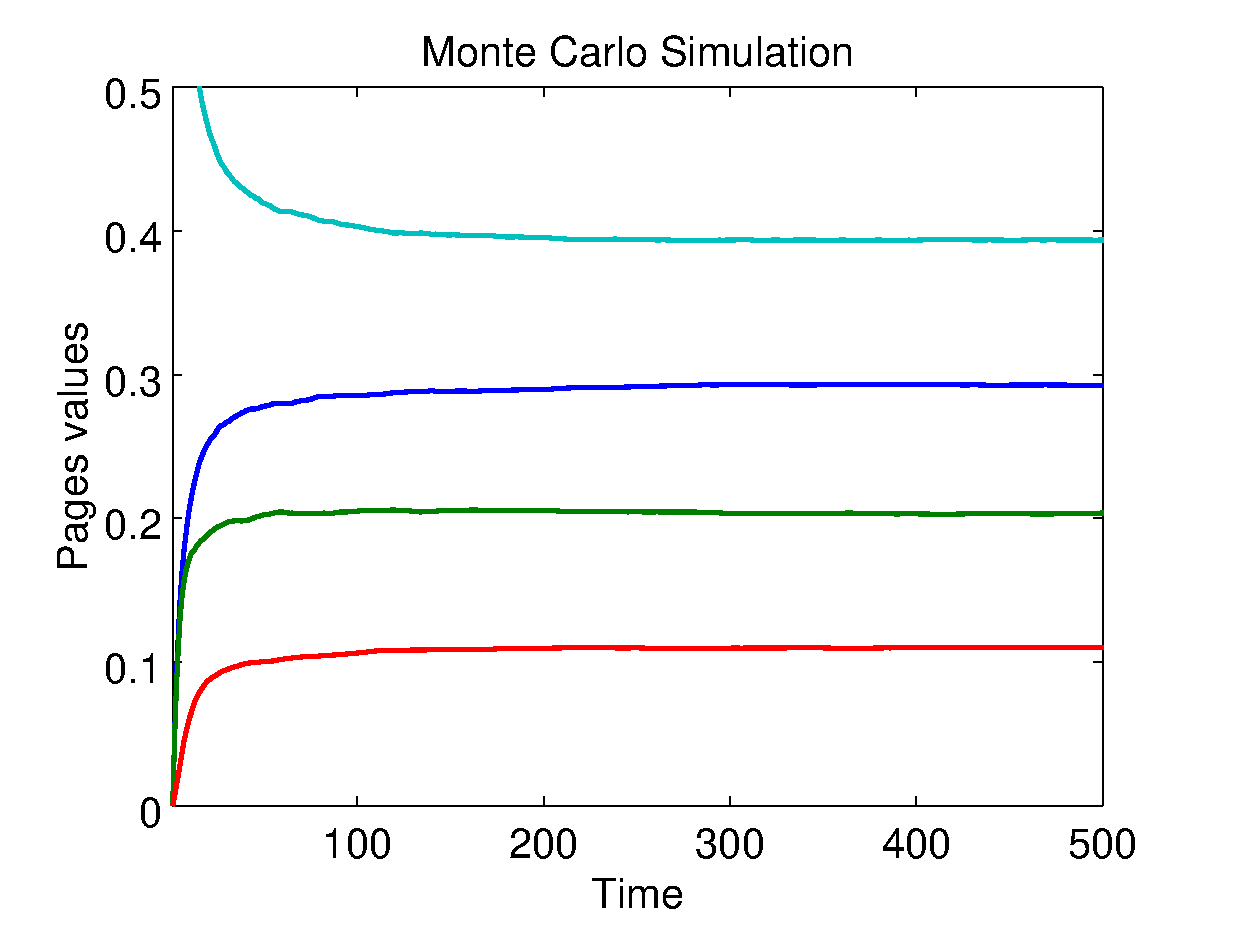
\includegraphics[scale=0.3]{imagens/montecarlo}
	\caption{Resultado das simulações com o método de Monte Carlo.}
	\label{montecarlo}
\end{figure}

Comparando a simulação em que usou-se do método de Monte Carlo com a simulação da média no tempo, observa-se que o gráfico do método de Monte Carlo possui uma curva mais suavizada, o que pode ser constatado nos resultados apresentados na figura \ref{montecarlo}. Além disso a evolução dos valores está mais bem definida, principalmente quando comparados ao valor final da distribuição limite.

\
\begin{figure}[!htb]
	\centering
	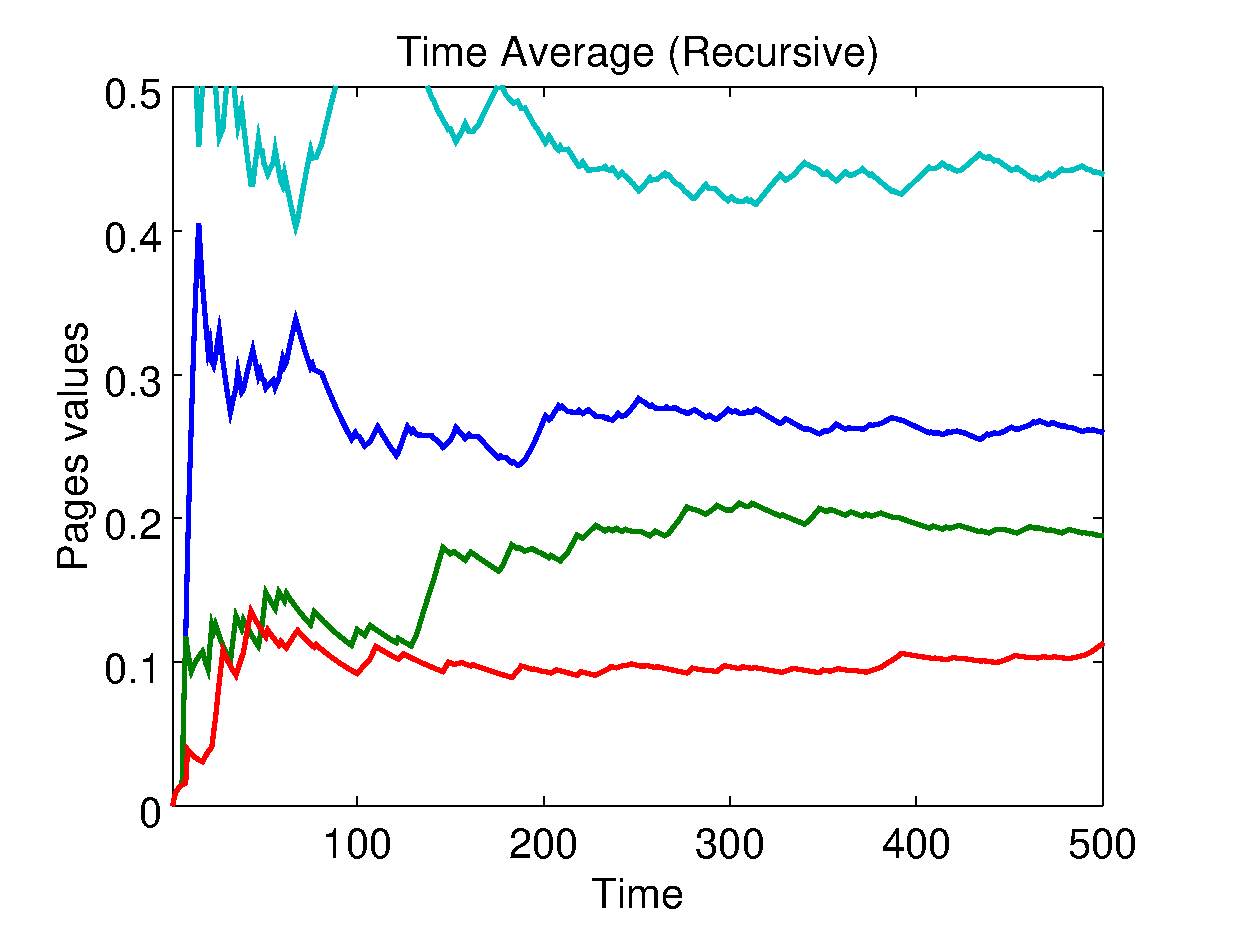
\includegraphics[scale=0.3]{imagens/timerecursive}
	\hspace{0.1cm}
	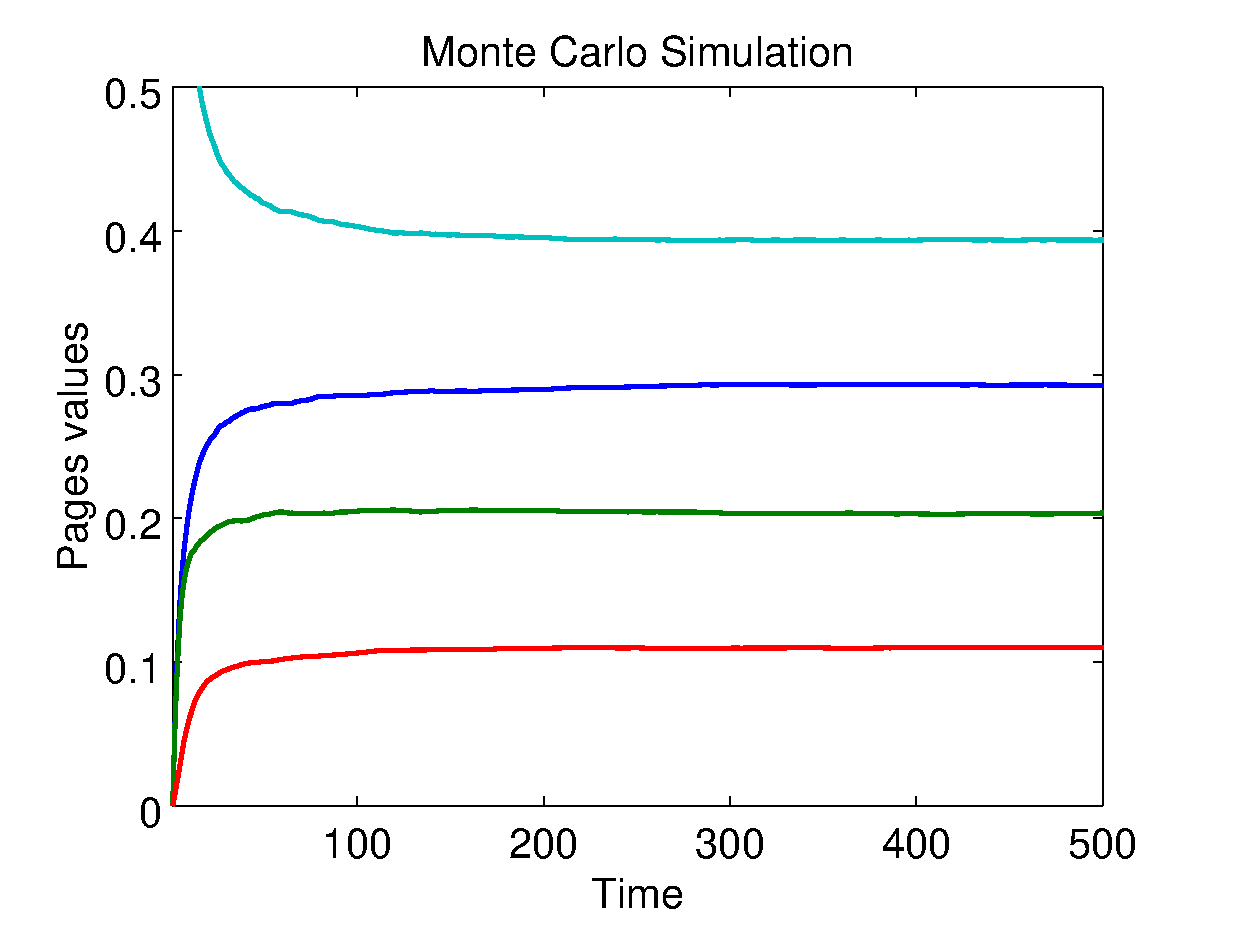
\includegraphics[scale=0.3]{imagens/montecarlo}
	\caption{Comparação entre a média no tempo do modelo distribuído e o método de Monte Carlo.}
	\label{timemonte}
\end{figure}

E ainda comparando os resultados da simulação com Monte Carlo e da simulação do \textit{Power Method} \ref{powermonte}, nota-se que os valores finais estão de acordo com os alcançados no modelo do \textit{Power Method}, o que sugere que o modelo é válido.

\
\begin{figure}[!htb]
	\centering
	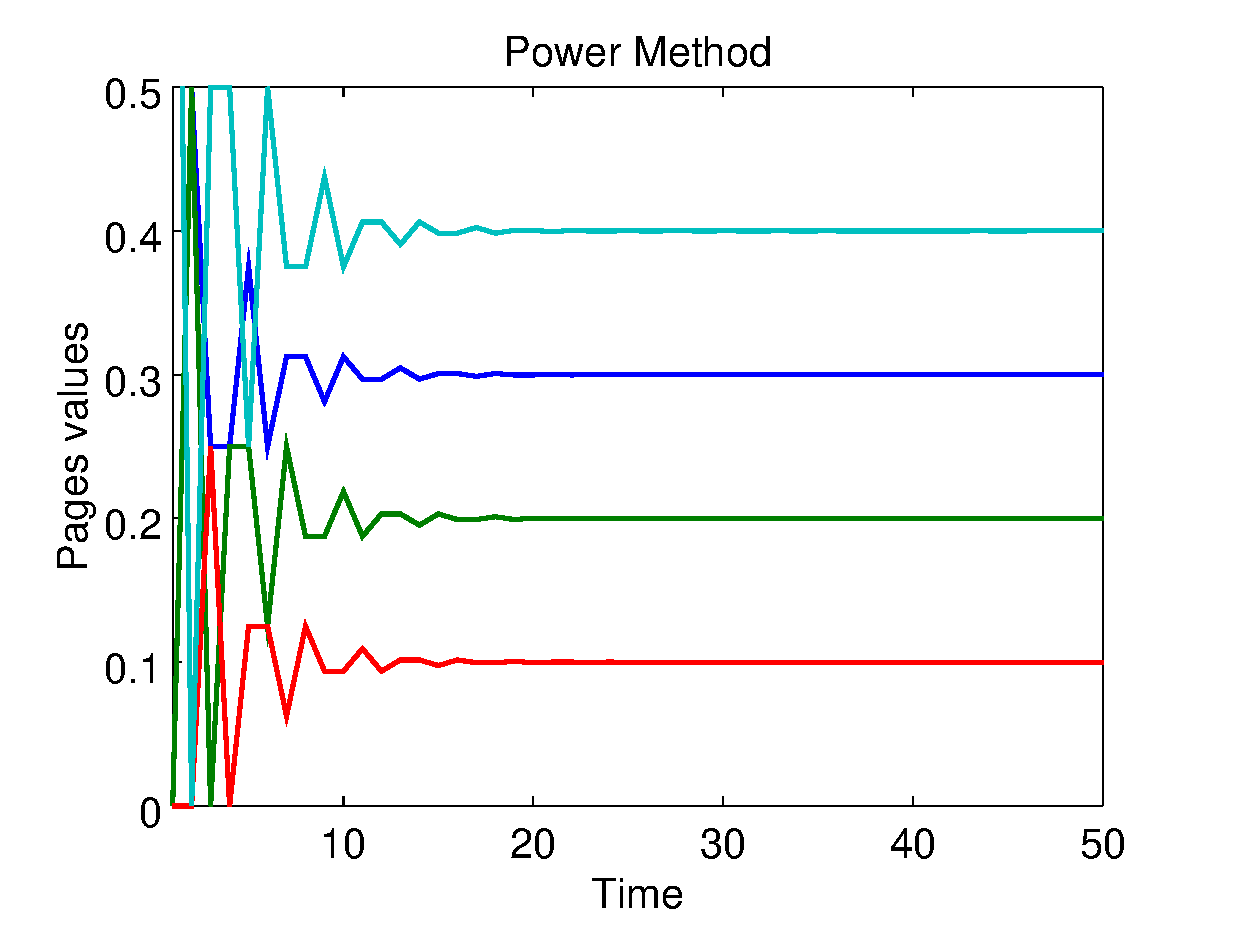
\includegraphics[scale=0.3]{imagens/powermethod}
	\hspace{0.1cm}
	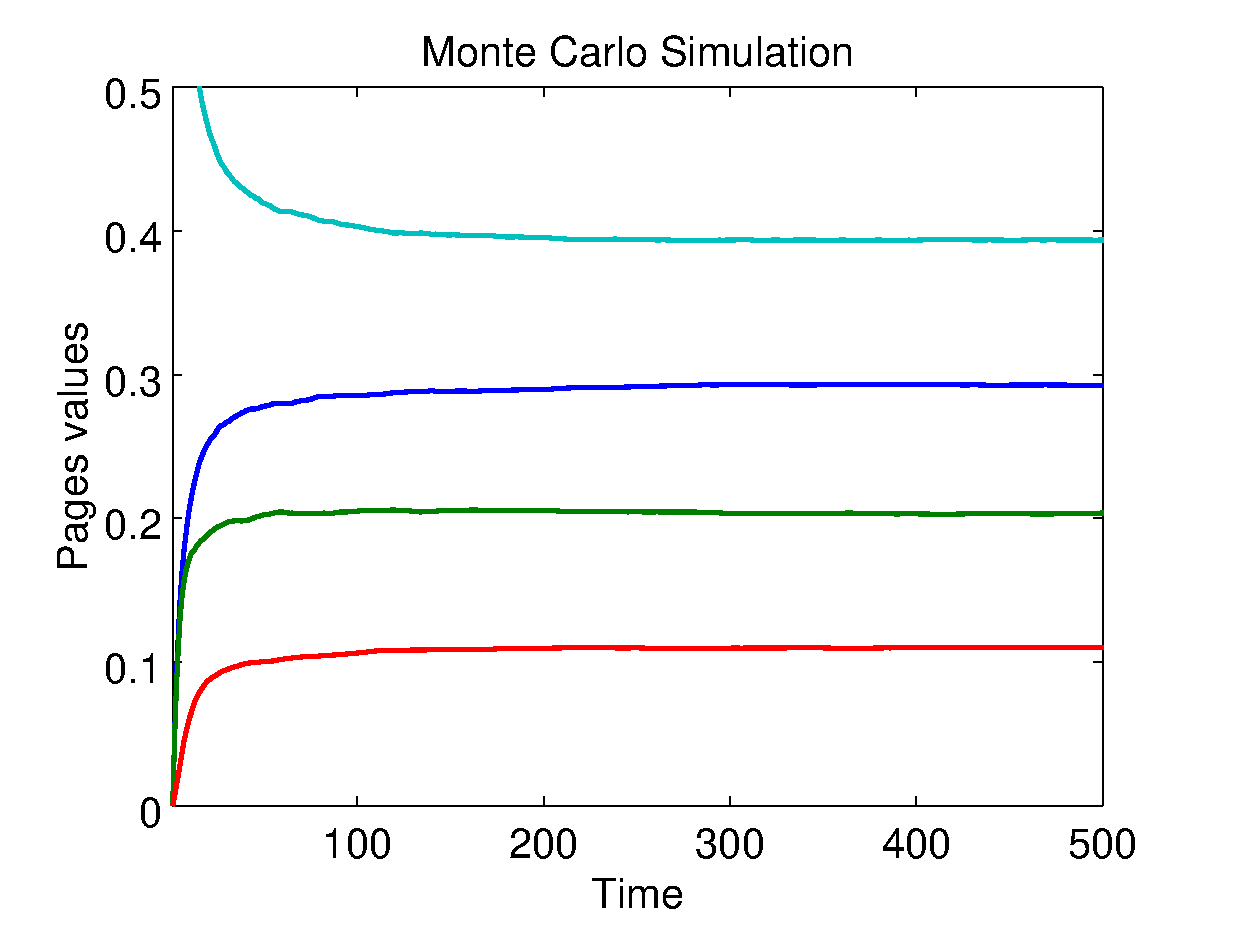
\includegraphics[scale=0.3]{imagens/montecarlo}
	\caption{Comparação entre os resultados do \textit{Power Method} e os obtidos com o método de Monte Carlo.}
	\label{powermonte}
\end{figure}

%%%%%%%%%%%%%%%%%%%%%%%%%%%%%%%%%%%%%%%%%%%%%%%%%%%%%%%%%%%%%%%%%%%%%%%%%%%%%%%%
\section*{Considerações Finais}

%Retornar o assunto principal.
Desde o início das pesquisas em desenvolvimento de ferramentas de busca em 1994, conseguir fazer um ranqueamento de páginas \textit{Web} de acordo com os interesses do usuário tem sido a parte mais desafiadora no desenvolvimento desses sistemas. Foi talvez por partir desse problema, e com uma boa solução, que o buscador Google obteve tamanho sucesso desde sua criação ao final da década de 90. As técnicas e modelos por trás do ranqueamento desse conjunto de documentos foram publicadas e, desde então, a comunidade científica tem trabalhado na pesquisa de novos modelos para tornar o cálculo do \textit{PageRank} mais eficiente.

O cálculo do \textit{PageRank} pode ser representado por diversos modelos, mas de forma geral é apresentado como uma equação de diferença, com algumas modificações na matriz de transição, a fim de tratar possíveis problemas de convergência. Os modelos e as propostas mais recentes do algoritmo estão voltados para o problema da distribuição do cálculo do ranquemento, no intuito de torná-lo cada vez mais eficiente. Mas a atenção ao algoritmo não tem por fim somente o ranqueamento de páginas \textit{Web}, a ideia do cálculo do \textit{PageRank} pode ser aplicada a diversos outros problemas.

%O que conclui-se do trabalho, objetivo geral e contribuições. Porque o meu trabalho é importante?
Durante o trabalho foi realizada uma revisão dos modelos propostos para o algoritmo do \textit{PageRank} na literatura. De forma que, inicialmente fosse efetuado um estudo dos modelos matemáticos por trás do algoritmo e em seguida fossem realizadas as simulações. Também para que fossem compreendidos os modelos matemáticos por trás do algoritmo, foi realizado um estudo sobre questões relacionadas a sistemas dinâmicos, sistemas estocásticos e probabilidade.

%Indicar trabalhos futuros a serem desenvolvidos.
Neste trabalho ainda pretende-se utilizar outros métodos válidos na simulação do \textit{PageRank}. Como a cada ano novos artigos são publicados no tema, novos modelos e técnicas estão sempre sendo publicados pela comunidade científica. Porém uma atenção maior seria dada a modelos agregados de cadeias de Markov, e problemas de consenso. E ainda como uma continuação deste trabalho, poderia ser feita uma implementação com \textit{links} já coletados por um \textit{Web Crawling}. De forma a por em prática os modelos num ambiente real e usando-se de técnicas de computação distribuída, afim de otimizar o cálculo e por em prática os algoritmos distribuídos. Além de usar outras linguagens de programação, como C e C++, por questões de desempenho e por serem mais adequadas a implementações em \textit{clusters}.

%%%%%%%%%%%%%%%%%%%%%%%%%%%%%%%%%%%%%%%%%%%%%%%%%%%%%%%%%%%%%%%%%%%%%%%%%%%%%%%%
\bibliographystyle{plain}
\bibliography{ref}

%%%%%%%%%%%%%%%%%%%%%%%%%%%%%%%%%%%%%%%%%%%%%%%%%%%%%%%%%%%%%%%%%%%%%%%%%%%%%%%%
\end{document}